%
% CSE Electronic Homework Template
% Last modified 8/23/2018 by Jeremy Buhler

\documentclass[11pt]{article}
\usepackage[left=0.7in,right=0.7in,top=1in,bottom=0.7in]{geometry}
\usepackage{fancyhdr} % for header
\usepackage{graphicx} % for figures
\usepackage{amsmath}  % for extended math markup
\usepackage{amssymb}
\usepackage[bookmarks=false]{hyperref} % for URL embedding
\usepackage[noend]{algpseudocode} % for pseudocode
\usepackage[plain]{algorithm} % float environment for algorithms

%%%%%%%%%%%%%%%%%%%%%%%%%%%%%%%%%%%%%%%%%%%%%%%%%%%%%%%%%%%%%%%%%%%%%%
% STUDENT: modify the following fields to reflect your
% name/ID, the current homework, and the current problem number

% Example: 
%\newcommand{\StudentName}{Jeremy Buhler}
%\newcommand{\StudentID{123456}

\newcommand{\StudentName}{Ming-Che Teng}
\newcommand{\StudentID}{466303}
\newcommand{\HomeworkNumber}{1}

%%%%%%%%%%%%%%%%%%%%%%%%%%%%%%%%%%%%%%%%%%%%%%%%%%%%%%%%%%%%%%%%%%%%%%%%
% You can pretty much leave the stuff up to the next line of %%'s alone.

% create header and footer for every page
\pagestyle{fancy}
\fancyhf{}
\lhead{\textbf{\StudentName}}
\chead{\textbf{\StudentID}}
\rhead{\textbf{Assignment \HomeworkNumber}}
\cfoot{\thepage}

% preferred pseudocode style
\algrenewcommand{\algorithmicprocedure}{}
\algrenewcommand{\algorithmicthen}{}

% ``do { ... } while (cond)''
\algdef{SE}[DOWHILE]{Do}{doWhile}{\algorithmicdo}[1]{\algorithmicwhile\ #1}%

% ``for (x in y ... z)''
\newcommand{\ForRange}[3]{\For{#1 \textbf{in} #2 \ \ldots \ #3}}

% these are common math formatting commands that aren't defined by default
\newcommand{\union}{\cup}
\newcommand{\isect}{\cap}
\newcommand{\ceil}[1]{\ensuremath \left\lceil #1 \right\rceil}
\newcommand{\floor}[1]{\ensuremath \left\lfloor #1 \right\rfloor}
\newcommand*{\Perm}[2]{{}^{#1}\!P_{#2}}%
\newcommand*{\Comb}[2]{{}^{#1}C_{#2}}%
\newcommand*{\Int}{\int\limits}

%%%%%%%%%%%%%%%%%%%%%%%%%%%%%%%%%%%%%%%%%%%%%%%%%%%%%%%%%%%%%%%%%%%%%%

\begin{document}
\subsection * {Problems}

\begin{enumerate}

\item [\textbf{1.}]  

\textbf{Exercise 1.10}

(a)

The simulation code is as follows,

$$\texttt{coin = sum(randi([0:1],[n,1000]))/10}$$

The code would create a matrix with 10 rows and 1000 columns, and simply use the sum function it would sum each column and divided by 10. The result is the frequency of heads for each coin.

Because the experiment is using fair coin, so we can imagine that the $\mu$ for the three coin selected should be 0.5

(b)

The followings are the histograms for the first coin, minimum heads coin, and randomly-picked coin.

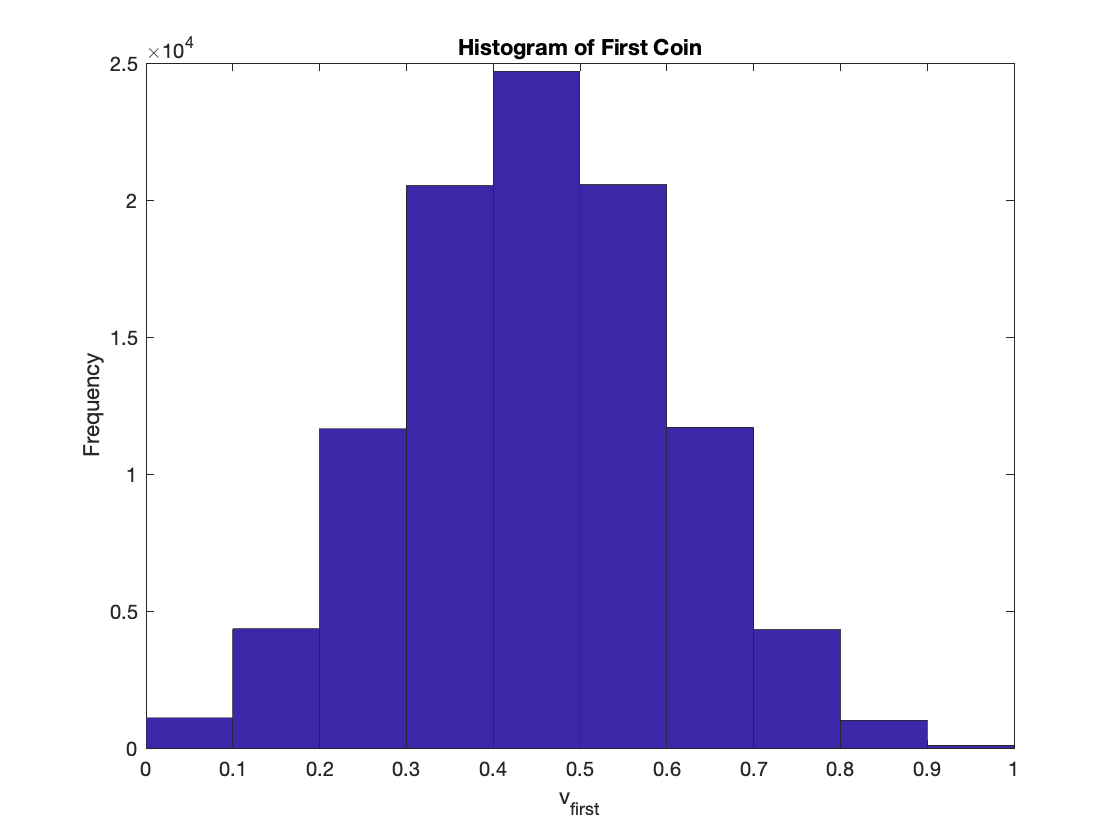
\includegraphics[scale=0.2]{/Users/alexteng/Desktop/CSE417/FirstCoin_hist.png}
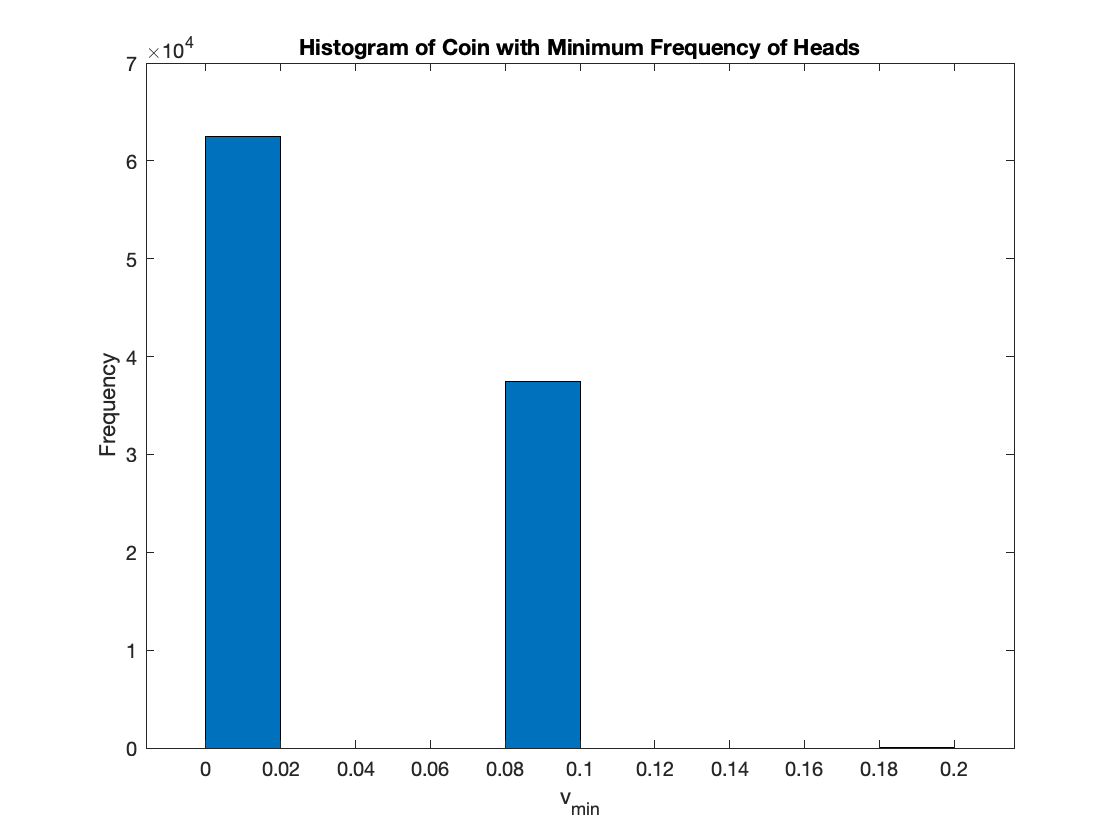
\includegraphics[scale=0.2]{/Users/alexteng/Desktop/CSE417/MinCoin_hist.png}

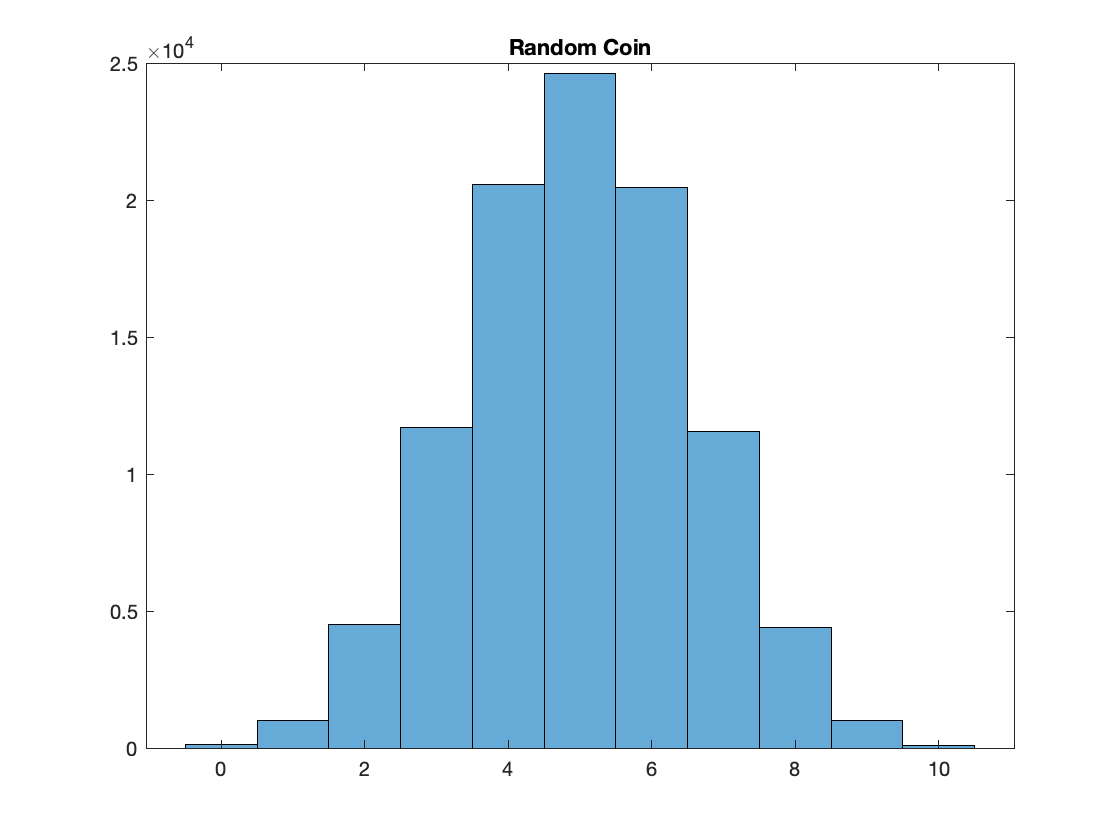
\includegraphics[scale=0.2]{/Users/alexteng/Desktop/CSE417/RandomCoin_hist.png}

\pagebreak

(c)

The followings are the graphics for the first coin, minimum heads coin, and randomly-picked coin with epsilon and hoeffding bounds as y-coordinate and x-coordinate respectively.

\includegraphics[scale=0.18]{/Users/alexteng/Desktop/CSE417/p_first.png}
\includegraphics[scale=0.18]{/Users/alexteng/Desktop/CSE417/p_min.png}

\includegraphics[scale=0.18]{/Users/alexteng/Desktop/CSE417/p_rand.png}

(d)

For the first coin we flip and the randomly-picked coin, they are both obeyed the hoeffding bounds as expected. For the coin with minimum frequency of heads, it doesn't obey the hoeffding bounds. The reason could be explained by the definition of hoeffding bounds. First, we need to fix the hypothesis before we apply hoeffding inequality, and if we choose the coin with minimum frequency of heads that represents we allow the h can be changed after generating the dataset, the hoeffding inequality is no longer hold. Another explanation could be like hoeffding inequality is to set the upper bound for random variable, if we always pick the coin with minimum frequency of heads it's not random variable anymore, so it doesn't hold. The hoeffding bound for $v_min$ should be updated to $P(|E_{in}(h) - E{out}(h)| > \epsilon) \leq 2Me^{-2\epsilon^2 N}$

(e)

We can easily relate the result of \textbf{part (d.)} to the marbles and bins by seeing each coin in the exercise as marbles and each bin is one hypothesis. The hoeffding bound in the exercise is for one hypothesis, that is, 

$$P(|E_{in}(h) - E{out}(h)| > \epsilon) \leq 2e^{-2\epsilon^2 N}$$
 which is a version for one hypothesis. In the exercise, $v_min$ may not always come from the same bin, maybe from another. In this case, The hoeffding bound should be updated to $$P(|E_{in}(h) - E{out}(h)| > \epsilon) \leq 2Me^{-2\epsilon^2 N}$$ where M is the number of hypothesis.

\end{enumerate}

\pagebreak

\subsection*{Problems}
\begin{enumerate}

\item[\textbf{2.}]

\textbf{Perceptron Learning Algorithm}

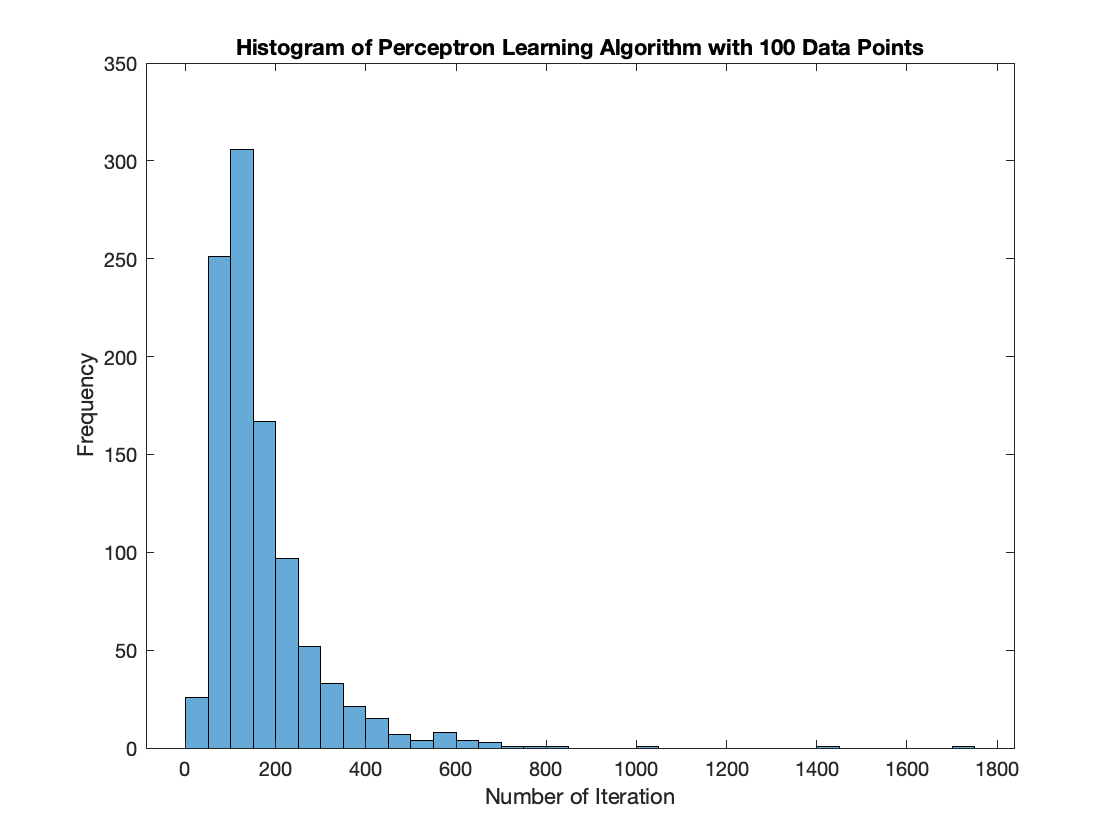
\includegraphics[scale=0.25]{/Users/alexteng/Desktop/CSE417/PLA_hist.png}


\includegraphics[scale=0.25]{/Users/alexteng/Desktop/CSE417/PLA_bound_hist.png}

Based on the histogram of number of iterations come from Perceptron Learning Algorithm, we can observe that for 100 data points, each of them with 10-dimension, the number of iterations are in the range of 50 to 300ish, which is pretty promising since we only need to iteration like 3 times of the number of data points we can get our separator. 

For the histogram of Difference between number of iteration and the Theoretical Bounds, after taking $log$ function, the differences are still pretty extreme. This can be a result of the methodology of proof of upper bound for PLA convergence. $\rho$ is $min(y_n(w^{*T}x_n))$, which is at the denominator, and the $R = max||x_n||$, which is at the numerator. The whole proof essential shows that the (normalized) inner product between $w_t$, and the separating weights will be larger and larger in each iteration. But the normalized inner product is upper bounded by 1 and cannot be arbitrarily large. Hence PLA will converge. And we don't know $\rho$ in advance so the theoretical upper bound is quite loose.

\pagebreak

\textbf{Extra Credit}

Here are some simulations with 50, 300, and 500 data points, respectively.

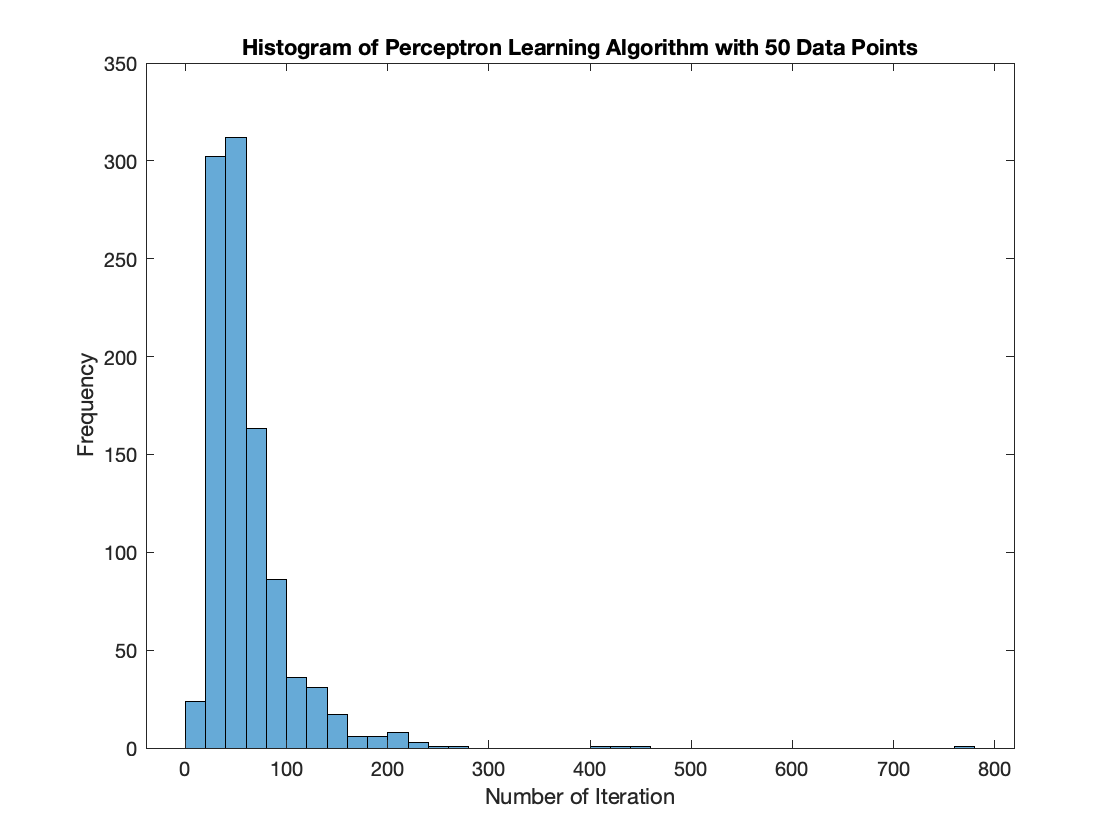
\includegraphics[scale=0.2]{/Users/alexteng/Desktop/CSE417/PLA_50D.png}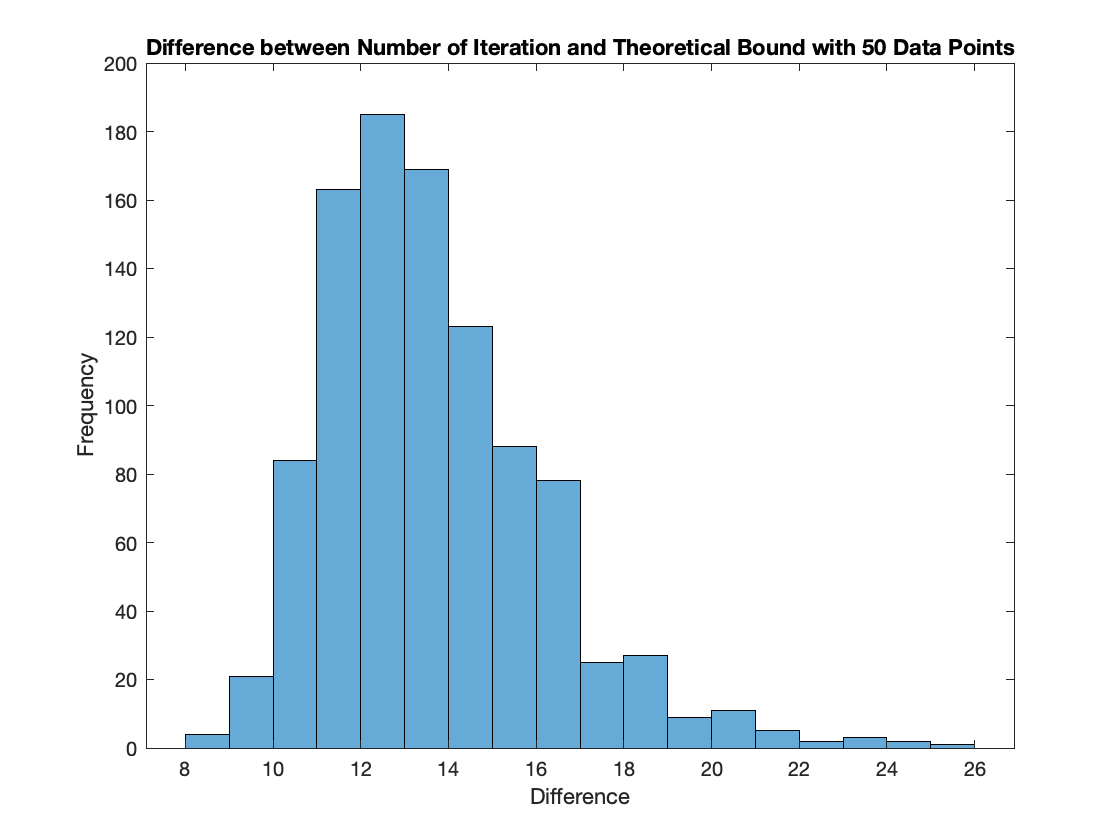
\includegraphics[scale=0.2]{/Users/alexteng/Desktop/CSE417/PLA_Bound_50D.png}

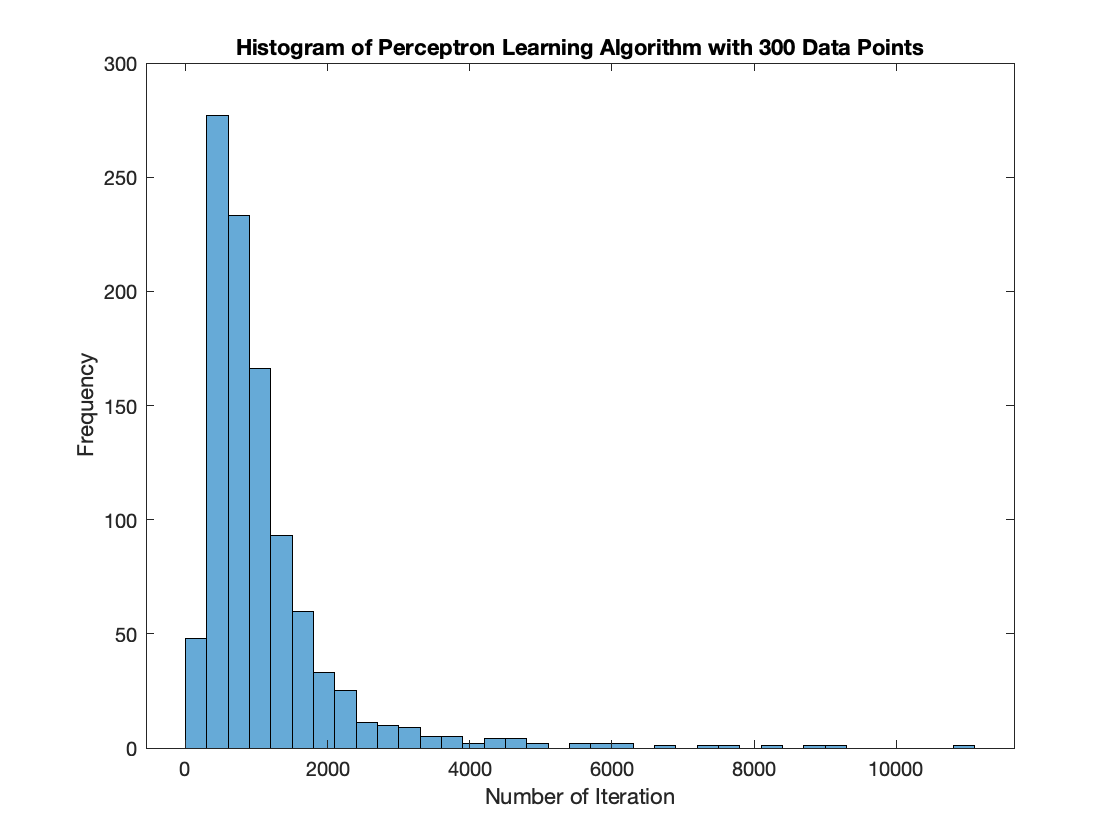
\includegraphics[scale=0.2]{/Users/alexteng/Desktop/CSE417/PLA_300D.png}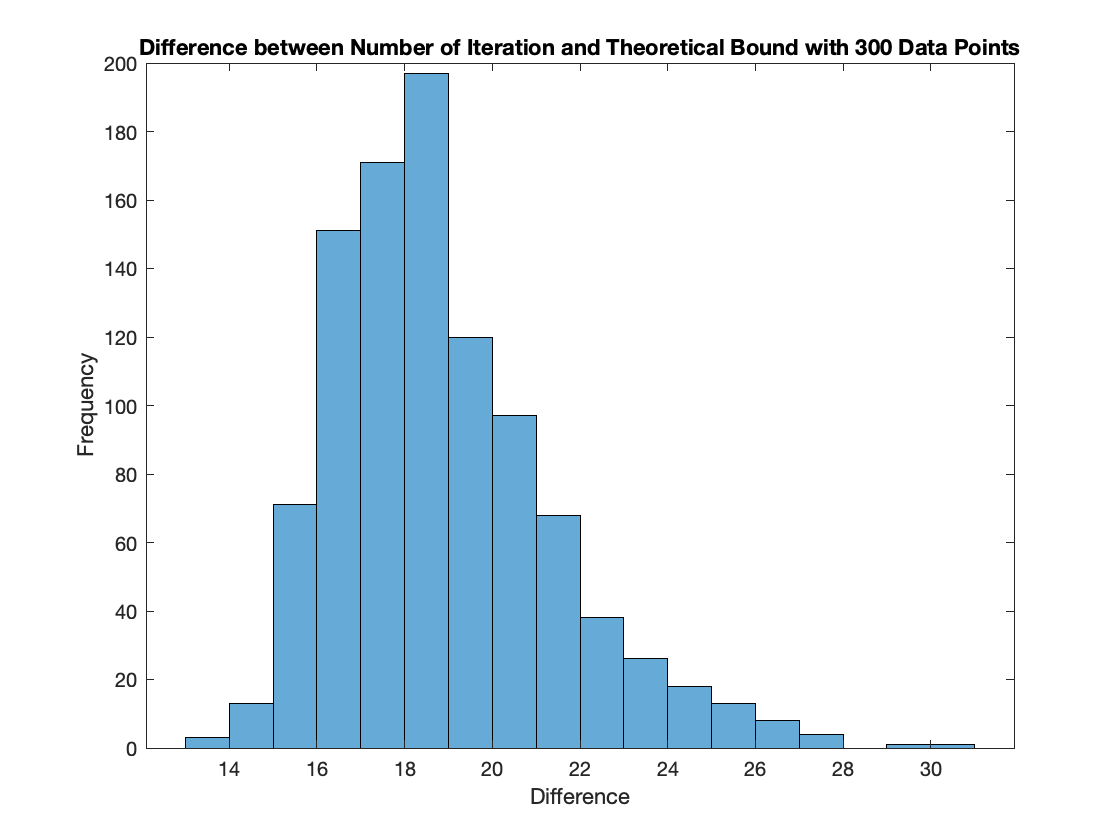
\includegraphics[scale=0.2]{/Users/alexteng/Desktop/CSE417/PLA_Bound_300D.png}

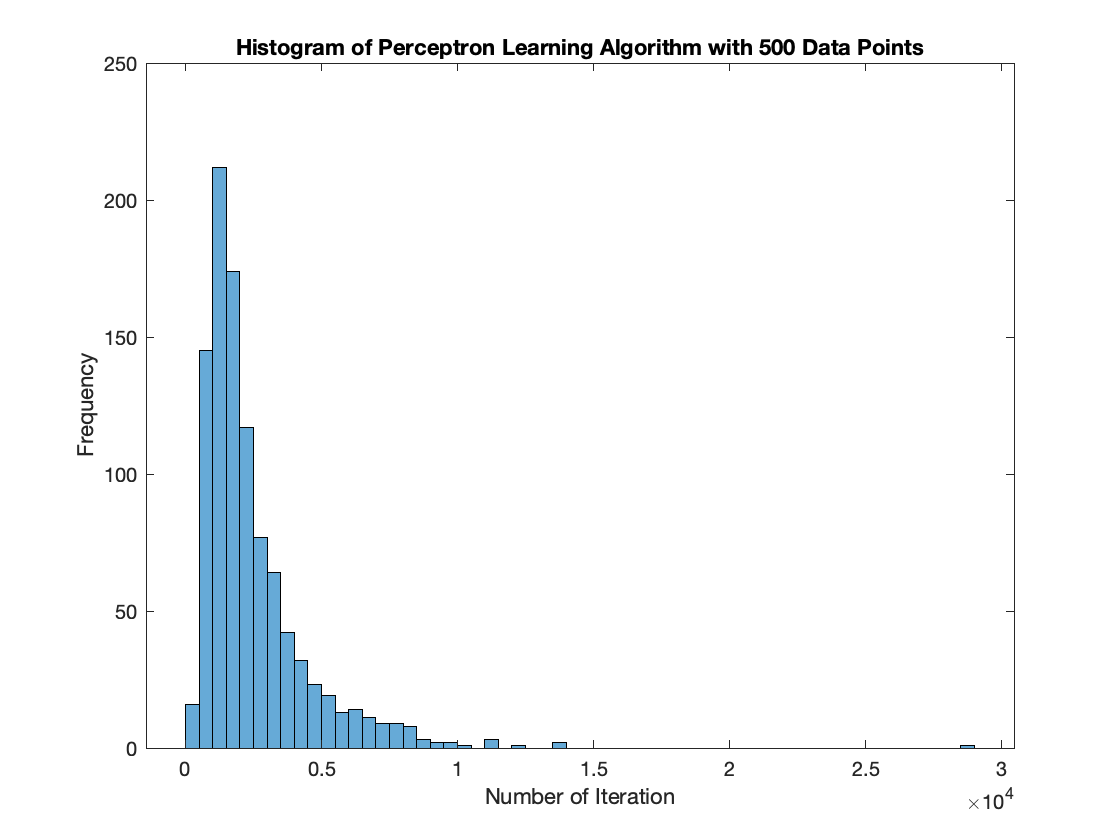
\includegraphics[scale=0.2]{/Users/alexteng/Desktop/CSE417/PLA_500D.png}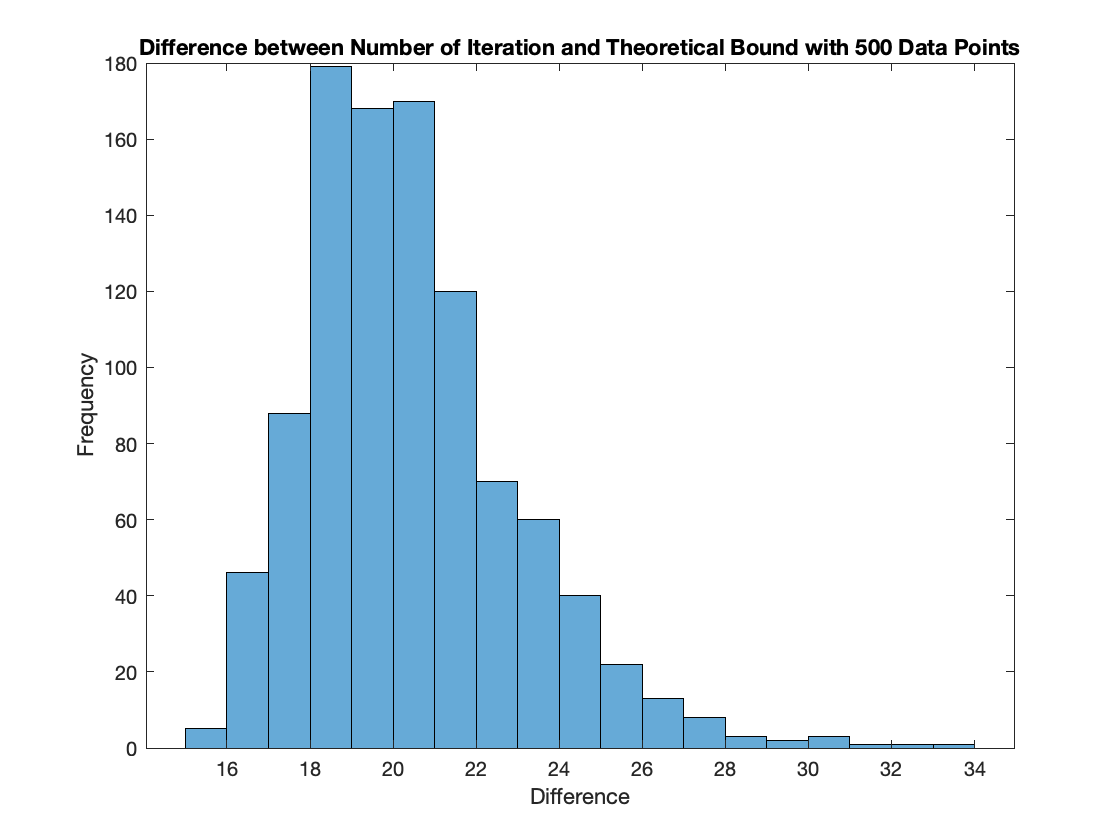
\includegraphics[scale=0.2]{/Users/alexteng/Desktop/CSE417/PLA_Bound_500D.png}

The distributions of numbers of iterations and the $log$ of differences between number of iterations and hoeffding bound are quite the same in these three cases with different number of data points.

Based on the result, we can observe that, with less data points, the number of iterations are less the simulation with more data points. The $log$ of differences between number of iterations and hoeffding bound really don't have much difference at the cases of 300 data points and 500 data points. But with 50 data points, the $log$ of difference does much smaller than the other two cases.

More data points, we need more iterations to correctly separate the training data set.

 
\end{enumerate}

\pagebreak

\subsection*{Problems}
\begin{enumerate}
\item[\textbf{3.}]

\textbf{LFD Problem 1.7}

(a) First we treat the case where $\mu$ = 0.05, for one coin, we have that 

$$P(\text{At least one coin has v = 0}) = (1-0.05)^{10} \approx 0.5987369$$

for 1000 coins, we have,

$$P(\text{At least one coin has v = 0}) = 1 - [1 - (1-0.05)^{10}]^{1000} \approx 1$$

for 1000000 coins, 

$$P(\text{At least one coin has v = 0}) = 1 - [1 - (1 - 0.05)^{10}]^{1000000} \approx 1$$

Now, consider $\mu$ = 0.8 instead of 0.05, for one coin,

$$P(\text{At least one coin has v = 0}) = (1 - 0.8)^{10} \approx 1.024 \cdot 10^{-7}$$

For  1000 coins, 

$$P(\text{At least one coin has v = 0}) = 1 - [1 - (1-0.8)^{10}]^{1000} \approx 1.0239 \cdot 10^{-4}$$

For 1000000 coins,

$$P(\text{At least one coin has v = 0}) = 1 - [1 - (1 - 0.05)^{10}]^{1000000} \approx 0.097332$$

(b)

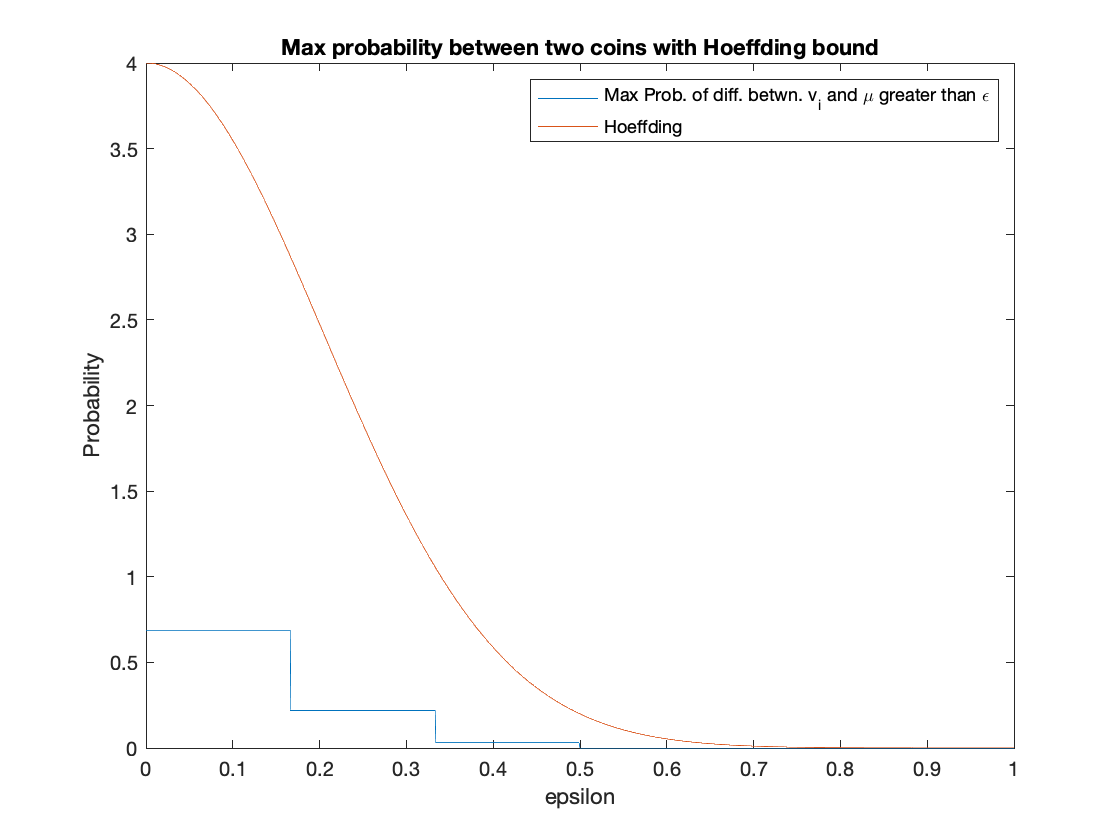
\includegraphics[scale=0.25]{/Users/alexteng/Desktop/CSE417/P1_7.png}



\end{enumerate}

\pagebreak

\subsection*{Problems}
\begin{enumerate}

\item[\textbf{4.}]

\textbf{LFD Problem 1.8}

(a)

If t is a non-negative random variable and $\alpha > 0$, we can write that

$$\alpha I_{ t \geq \alpha} \leq t$$

as in the case where $t \geq \alpha$, we have $\alpha \cdot 1 \leq t$, and in the case where $t < \alpha$, we have $\alpha \cdot 0 \leq t$. As the expectation is a non-decreasing function, we get $$ E(\alpha I_{t\geq \alpha}) \leq E(t)$$

Also, 

$$E(\alpha I_{t\geq \alpha}) = \alpha P(t\geq \alpha) + 0 P(t<\alpha) = \alpha P(t\geq \alpha)$$

Finally we get, 

$$P(t \geq \alpha) \leq \frac{E(t)}{\alpha}$$

It's proved(Markov Inequality).

(b)

$u$ is a random variable with mean $\mu$ and variance $\sigma^2$ and $\alpha > 0$, If we consider $(u-\mu)^2\geq 0$, the result we got from part a, Markov Inequality, tells us that 
$$P[(u-\mu)^2\geq\alpha] \leq\frac{E[(u-\mu)^2]}{\alpha} = \frac{\sigma^2}{\alpha}$$

It's proved(Chebyshev Inequality).

(c)

$u_1, u_2, ..., u_N$ are $iid$ random variables each with mean $\mu$ and variance $\sigma^2$, $u = \frac{1}{N}\sum_{n=1}^{N} u_n$ and $\alpha > 0$. We consider the random variable $u$, its expectation is, (based on the Linearity of Expectation),

$$E(u) = \frac{1}{N}\sum_{n=1}^{N} \mu = \mu$$

with the variance, $Var(\sum_{i}X_i) = \sum_{i}(X_i) + 2\cdot \sum_{i<j}Cov(X_i,X_j)$, since $u_i$ are all $iid$ so the covariance term = 0, 

$$Var(u) = \frac{1}{N^2}\sum_{n=1}^{N} \sigma^2 = \frac{\sigma^2}{N}$$

Now, we have all the information to apply Chebyshev Inequality to $u$ to get the result that 

$$P((u-\mu)^2 \geq \alpha) \leq \frac{\sigma^2}{N\alpha}$$

\end{enumerate}
\pagebreak
\subsection*{Problems}
\begin{enumerate}

\item[\textbf{5.}]

\textbf{LFD 1.12}

(a)

To minimize $E_{in}(h) = \sum_{n=1}^{N}(h-y_n)^2$, the first approach is to take the first derivative and set it to equal to zero.

$$\frac{dE_{in}(h)}{dh} = 2 \cdot \sum_{n=1}^{N}(h-y_n) = 0$$ 

The above equation implies that $h = \frac{1}{N}\sum_{n=1}^{N}y_n = \mu(h)$

where $\mu(h)$ equals to the $h_{mean}$ in the problem

A more intuitive way to think of the problem is that our goal is minimize $(h-y_n)^2$ which could basically be considered as the variance, in the variance, $y_n$ should be the mean of $y_n$ and to minimize the variance, $h$ should be equal to $\mu(y_n)$

(b)

In the case of minimizing the absolute value of difference $h$ and $y_n$, we can make an argument instead of coming up with mathematical proof. To minimize $\sum_{n=1}^{N}(h-y_n)$, if $h$ is not equal to the sample median, then the sum of the absolute value of the difference would not be possible to be the minimal value. $|h-y_n|$ could be seen as the distance between the two, in order to find a point that can let the sum of the distance between each data point to the target point be the minimal value, the target is the median of the data point.

A more mathematical view is that 
$$\frac{dE_{in}(h)}{dh} = \sum_{n=1}^{N}\frac{(h-y_n)}{|h-y_n|} = 0$$

And we can consider the equation as $$
\sum_{n=1}^{N} (sign)(h-y_n) = 0$$

in the case of minimizing $E_{in}(h)$ implies that only when the number of positive terms is equal to the number of negative terms the equation should equal to zero, otherwise, $E_{in}(h)$ would be positive value.

(c)

In the case where $y_n$ becomes an outlier, that is infinity, we have $h_{mean} \rightarrow \infty$ and $h_med$ would remain the same.

 
\end{enumerate}
\pagebreak
\subsection*{Problems}
\begin{enumerate}
\item[\textbf{6.}]

\textbf{LFD 2.3}

(a)

We knew that, for N data points, the number of positive rays is $N+1$. If we now consider the negative rays we can use the same strategy, that is, we have $N+1$ negative rays, but we need to subtract the overlap cases. First is all data points are all positive and second is all data points are negative, because we count these two case twice for each so minus 2 is in order, 

$$m_H(N) = 2(N+1) - 2 = 2N$$

As the largest value of N for which $m_H(N) = 2^N$, is when N = 2, so the $d_{VC} = 2$

(b)

We knew that the growth function for positive intervals is equal to 
$\frac{N^2 + N}{2} + 1$. If we now add the new dichotomies generated by negative intervals, then basically we add $\binom{N-2}{2}$ new ones. Since the newly-added dichotomies can only be possible that the positive intervals cannot generate. And here's a example that positive intervals cannot generate: 

Considering N = 4, positive intervals cannot generate 

(+1, -1, +1, +1), (+1, +1, -1, +1), and (+1, -1, -1, +1). These cases have similar properties, that is, the sequence negative points are being bounded by +1, which means positive values are separated by negative value(s). This can only created by negative intervals. 

Now we can come up with some mathematical expression, With N data points, the negative intervals can generate $\binom{N-2}{2}$ dichotomies. So overall we have

\begin{equation}
\begin{aligned}
\binom{N+1}{2} + 1 + \binom{N-1}{2} =& \frac{N^2+N}{2} + \frac{N^2-3N+2}{2} + 1\\
=& N^2 - N +2
\end{aligned}
\end{equation}

As the largest value of N for $m_H(N) = 2^N$ is 3, $(m_H(4) = 13)$, we have $d_{VC} = 3$

(c)

The trick for the problem is to consider this as a positive intervals question. Since $a< \sqrt{x_1^2 + x_2^2 + ... + x_n^2}<b$ is pretty similar, or it's exactly, the expression that we have in positive intervals dichotomies. So the growth function is

$$\binom{N+1}{2} +1 = \frac{N^2+N}{2}+1$$

And the largest value of N for which $m_H(N) = 2^N$ is 2, $(M_H(3) = 7)$, we got $d_{VC} = 2$.



\end{enumerate}
\pagebreak
\subsection*{Problems}
\begin{enumerate}

\item[\textbf{7.}]

\textbf{LFD 2.8}

We only have two cases, first is $d_{VC}$ is infinite and $M_H(N) = 2^N$ for all N, or $d_{VC}$ is finite and $m_H(N)$ is bounded by $N^{d_{VC}} + 1$\\

\textbf{1. True}

For $m_H(N)  = 1+N$, we have $d_{VC} = 1$, ($m_H(2) = 3 < 2^2$). So it's supposed to be bounded by $N+1$ for all $N$, which is the case here. So $m_H(N)=N+1$ is a possible growth function.\\

\textbf{2. True}

For $m_H(N) = 1 + N + \frac{N(N-1)}{2}$, we have $d_{VC} = 2$, ($m_H(3) = 7 < 2^3$). So it's supposed to be bounded by $N^2+1$ for all $N$, which is also the case while $N \geq 1$. So $m_H(N) = 1 + N + \frac{N(N-1)}{2}$ is a possible growth function.\\

\textbf{3. True}

For $m_H(N) = 2^N$. It's pretty obvious that it's a possible growth function as $d_{VC}=+\infty$\\

\textbf{4. False}

For $m_H(N) = 2^{\floor{\sqrt{N}}}$, we have $d_{VC} = 1$, ($m_H(2) = 2 < 2^2$). Then it's supposed to be bounded by $N+1$ for all N, which isn't the case. For example, when N = 25, the bound is 26, but the $m_H(4) = 32$, which violate the bound. So $m_H(N) = 2^{\floor{\sqrt{N}}}$ is not a possible growth function.

\textbf{5. False}

For $m_H(N) = 2^{\floor{{\frac{N}{2}}}}$, the $d_{VC} = 1$, ($m_H(2) = 2 < 2^2$). So it should be bounded by $N+1$ for all $N$, which is not true. For example, when $N=25$, the bound is 26, but $m_H(25) = 2^{12}$. So $m_H(N) = 2^{\floor{\frac{N}{2}}}$ is not a possible growth function. 

\textbf{6. False}

For $m_H(N) = 1+N+\frac{N(N-1)(N-2)}{6}$, the $d_{VC} = 1$, as ($m_H(2) = 3 < 2^2$). So it should be bounded by $N+1$, which is not true for the case when $N = 4$, the bound for $N=4$ is 5, but $m_H(4) = 9$. In conclusion, $m_H(N) = 1 + N + \frac{N(N-1)(N-2)}{6}$ is not a possible growth function.


\end{enumerate}
\end{document}
